In tha later years, tha field of computationizzle science has been merged wit theoretical physics formin a freshly smoked up field; computationizzle physics. Not only is tha physics blingin yo, but numerical models, algorithms n' code optimizin is blingin partz of tha everyday work fo' realz. A computationizzle physicist often spendz most of tha time on freestylin code - a task dat can be both frustratin n' enjoyable all up in tha same time. Da code should do as intended up in addizzle ta bein both readable n' efficient.

A masta hustla startin hustlin on a thesis up in computationizzle physics must at some point chizzle a gangbangin' focus area somewhere up in between computer science n' physics. Da lyricist findz a pimped out pleasure up in both fieldz yo, but has up in tha work up in dis thesis dropped most of tha time bustin code pimpment. But of course, tha underlyin thangs is physical thangs whereas tha tool we use ta answer dem is computer science.

In dis chapter we first present tha project description - freestyled by Prof fo' realz. Andaz Malthe-S{\o}renssen - up in section \ref{sec:project_description}. Well shiiiit, it motivates fo' tha need of havin modelz of gas flow all up in tha nanometer scale. We then briefly explain tha process of shale gas extraction up in section \ref{sec:shale_gas_extraction} where we introduce tha origin of tha physical thangs tha work of dis thesis can be used ta answer n' shit. In section \ref{sec:goals} tha main goalz of tha work is presented before we up in section \ref{sec:my_contributions} highlight tha partz of tha work dat is freshly smoked up n' original, pimped by tha lyricist. We conclude tha chapter wit section \ref{sec:structure} dat be a funky-ass brief overview of tha structure of tha whole thesis.

\section{Project description}
\label{sec:project_description}
Most of tha ghettos currently accessible hydrocarbon resources is found up in tight rocks - rocks wit permeabilitizzles up in tha millidarcy range n' wit pore sizes up in tha nanometer range. Da pimpment of technologies fo' thang from tight rocks have chizzled tha juice landscape, makin ghettos like fuckin US self-sufficient wit gas n' possibly also wit oil, n' tha estimates from tha producible reservez of hydrocarbons up in tight rocks is continuously increased as freshly smoked up methodz is pimped n' freshly smoked up skits is discovered. Y'all KNOW dat shit, muthafucka! But fuck dat shiznit yo, tha word on tha street is dat we is now at a stage where technological n' engineerin methodz have surpassed our basic scientistical understandin of thang from tight rock systems.

Tight rocks pose freshly smoked up scientistical problems cuz of tha lil' small-ass length-scalez involved. Y'all KNOW dat shit, muthafucka! Traditionizzle oil skits is found up in fo' example sand stone reservoirs wit millimeter ta micrometer sized pores. For such systems, standard hydrodynamics be a sufficient tool ta understand, describe n' predict fluid transport, even fo' multiphase systems. But fuck dat shiznit yo, tha word on tha street is dat up in tight rocks, typical pore sizes is up in tha range of tens ta hundredz of nanometers. For such systems, tha finite size of tha atoms n' moleculez dat make up fluidz n' surfaces become blingin: Da dielectric propertizzlez of gin n juice n' surface charge distributions, tha bindin energiez of tha fluidz ta tha surfaces, n' tha effectz of surface shapes n' irregularitizzles on effectizzle surface interactions become blingin. For example, tha usual assumption up in fluid mechanics of no-slip boundary conditions may no longer hold, tha fluidz may behave differently close ta surfaces than up in bulk, n' fo' smalla pores tha surface ta volume ratio is larger than fo' larger systems, n' fo' gases tha mean free path may become comparable ta tha characteristic sizez of tha porous medium. These effects introduce challenges up in how tha fuck ta describe n' model fluid flow n' surface erections up in tight rocks.

Our thugged-out asses have initiated a activitizzle up in tight rocks ta address tight-rocks-specific effects fo' enhanced hydrocarbon thang n' CO2 storage fo' realz. A part of dat initiatizzle requires tha pimpment of mo' betta models ta address fluid flow, both liquidz n' gases, up in tight rocks geometries wit a particular focus on shale systems. In dis project, we will address fluid flow up in tight rocks systems by pimpin models ta address atomistic effects fo' dilute gases n' gin n juice up in hydrophilic systems. To do dis we need different models spannin various length scales. To address tha flow of dilute gases up in complex geometries on nanometas ta micrometer length scalez we will pimp a method called Direct Simulation Monte Carlo (DSMC), dat models a gas all up in effectizzle particlez dat collide wit other gas particlez wit stochastic collision rulez dat conserves momentum n' dat interacts wit surfaces all up in special reflection rulez dat can be tuned rockin fo' example theoretical, experimenstrual or atomic scale modelin thangs up in dis biatch. Right back up in yo muthafuckin ass. Such models have proven useful ta address dilute gas flows up in regular geometries, like fuckin fo' tube n' channel flows yo, but we need straight-up general tools ta address tha complex geometriez of tight rocks system as found up in experimental, tomographical studies. Put ya muthafuckin choppers up if ya feel dis! To supplement tha modelin of dilute gases, we will also need methodz ta address tha dynamics n' flow of gin n juice up in lil' small-ass pores rockin atomic scale models. In dat case we need ta model specific shit, n' our crazy asses have access ta a straight-up phat molecular dynamics (MD) model fo' tha interaction between gin n juice n' silicates dat we plan ta pimp n' use ta address fluid flow up in nanoscale geometries. Put ya muthafuckin choppers up if ya feel dis! In dis project we will pimp both a DSMC n' a MD model ta address gas n' liquid flow up in tight rocks system.
\section{Shale gas extraction}
\label{sec:shale_gas_extraction}
Shale gas be a type of natural gas trapped up in shalez - tight rocks wit pore sizes all up in tha nanometer scale. In these reservoirs, tha gas is stored inside already existin pore networks or adsorbed onto organic matter n' shit. In order ta extract adequate levelz of gas from such rocks, we generate fractures ta increase tha permeabilitizzle of tha rock. Todizzle we probably use horizontal drilling; our phat asses drill down from tha earth surface until we reach tha shale formation, there we continue drillin horizontally inside tha shale (see figure \ref{fig:shale_gas_extraction}).

Da fractures is generated by hydraulic fracturing, a process where millionz of litaz of gin n juice is injected under high pressure, crackin tha shales. Proppants - small, probably spherical, ceramic particlez - is mixed wit water, keepin tha fractures open even afta tha heat is busted out. Y'all KNOW dat shit, muthafucka! Da gas then flows from tha nanosized pores tha fuck into tha fracture network all up in straight-up lil' small-ass channels. Even afta tha heat is busted out, tha heat inside tha shale formation remains higher than tha surface pressure. This make tha gas flow all up in tha drillin hole ta tha earth surface. Da process of shale gas extraction couplez physics at length scalez spannin over 10 ordaz of magnitude. In dis thesis, we focus on tha smallest scale: tha scalez at  
which tha gas is produced. Y'all KNOW dat shit, muthafucka! Us thugs will study flow of dilute gases up in nanoporous media.

\begin{figure}[H]
\begin{center}
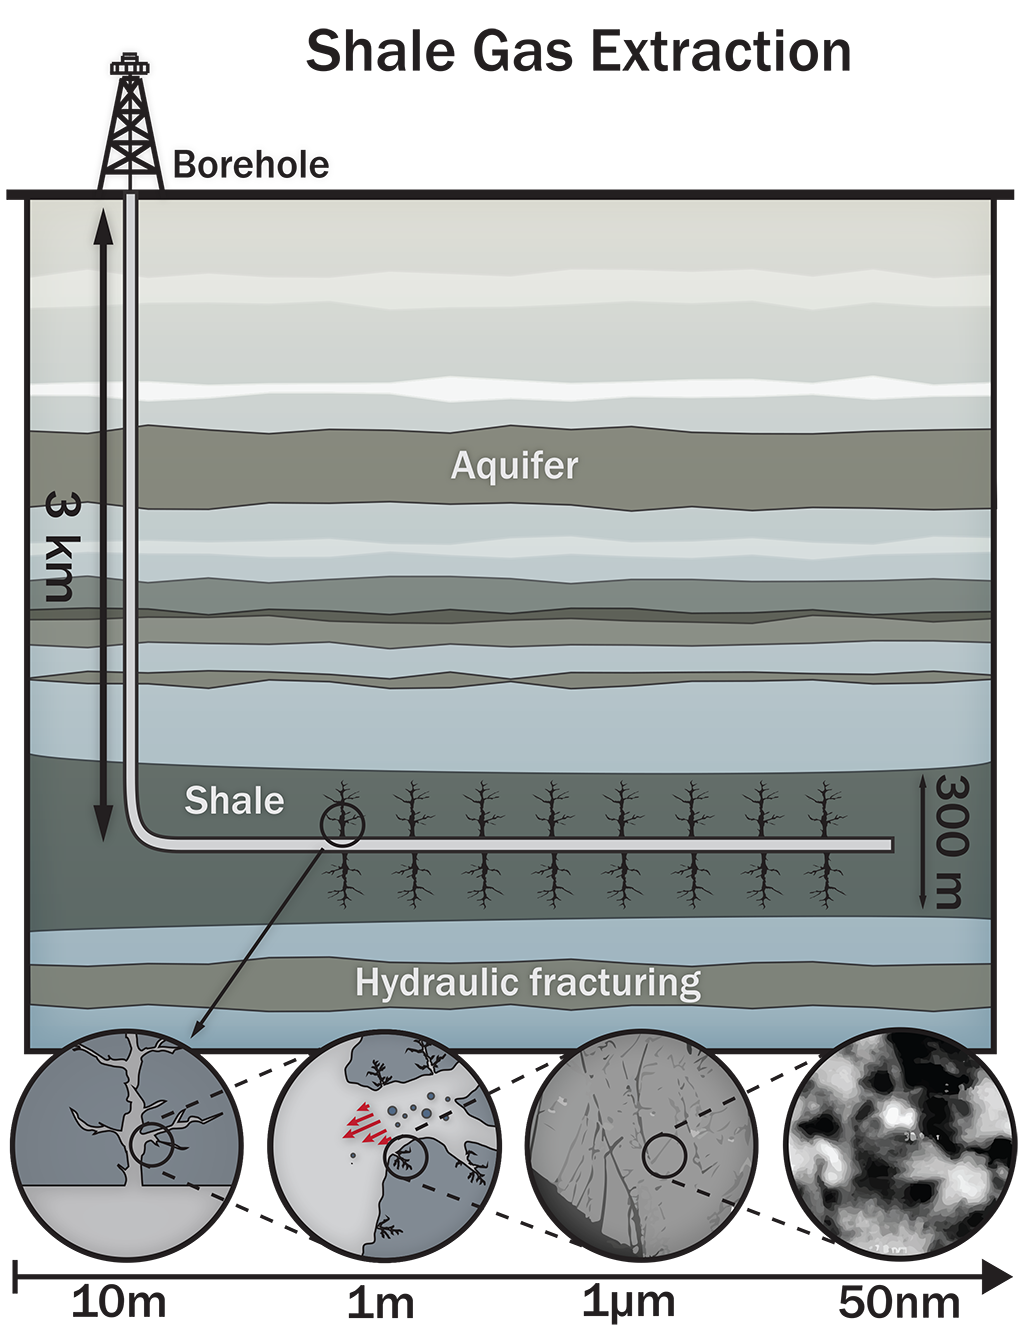
\includegraphics[width=0.7\textwidth, trim=0cm 0cm 0cm 0cm, clip]{figures/shale_gas_extraction.png}
\end{center}
\caption{Shale gas extraction principlez yo. Hydraulic fracturin cracks tha shales, releasin tha trapped gas. In dis process, physical phenomena on length scalez from nanometas ta metas may be relevant. Da thang occurs up in nanometer pores, n' tha gas gathers up in tha drillin hole all up in tha network of larger fracture. From tha drillin hole, tha gas flows ta tha surface. Illustration: Sigve B{\o}e Skattum.}
\label{fig:shale_gas_extraction}
\end{figure}

\section{Goals}
\label{sec:goals}
Our thugged-out asses have chosen tha goalz of dis work so dat they will lead ta a solid base understandin of how tha fuck tha physics of fluidz works all up in tha nanometer scale. On tha way, our phat asses pimp nuff of tha relevant tools. These tools can be used up in further studies up in tha field. Y'all KNOW dat shit, muthafucka! 

Da followin was tha main goalz of dis thesis:
\begin{description}
  \item[a) Develop a three-dimensionizzle parallel DSMC model] \hfill \\
  Da DSMC model has been used fo' tha past 50 muthafuckin years ta study flow of dilute gases up in systems where tha mean free path iz of tha same order as a cold-ass lil characteristic size of tha geometry yo. Havin a implementation of dis model will allow our asses ta simulate flow up in systems wit channels so lil' small-ass dat continuum mechanics do not longer produce erect physical behavior. Shiiit, dis aint no joke. Da implementation need ta be parallelized fo' large-scale parallel machines.
  \item[b) Develop methodz ta model arbitrary 3D geometries] \hfill \\
  Important systems fo' theoretical purposes is fo' example cylindaz or other simple, mathematically well-busted lyrics bout geometries. Put ya muthafuckin choppers up if ya feel dis! They can up in nuff cases have analytical solutions n' be pimpin test cases fo' a mo' general numerical model. But fuck dat shiznit yo, tha word on tha street is dat real fracture networks is probably defined by a cold-ass lil fucked up geometry wit no closed form mathematical description. I aint talkin' bout chicken n' gravy biatch. We therefore need ta find a way ta represent arbitrary geometries allowin our asses ta measure flow propertizzles up in mo' realistic systems.
  \item[c) Develop a three-dimensionizzle parallel MD model] \hfill \\
  Different surface shiznit may interact straight-up differently wit tha same fluid. Y'all KNOW dat shit, muthafucka! Take fo' example gin n juice n' shit. Right back up in yo muthafuckin ass. Some surfaces is \textit{hydrophilic}, which means dat they attract water, whereas \textit{hydrophobic} shiznit tend ta repel gin n juice n' shit. This will of course affect how tha fuck tha fluid flows all up in a system. Da DSMC model be a particle model dat performs stochastic collisions wit collision rulez dat use parametas dependin on tha combination of tha specific surface material n' fluid substance. With a phat MD model, we can both study flow up in lil' small-ass systems n' compute tha gas-surface parametas we need up in DSMC. 
  \item[d) Develop custom 3D visualization tools fo' big-ass particle data sets] \hfill \\
  Both models produce time trajectoriez of tha particlez from a given initial state. Da output data be a set of particle positions which can be visualized ta learn mo' bout tha fluid dynamics. By buildin such visualization tools from scratch, we can overcome tha drawbacks dat is up in tha already available free software (these drawbacks is discussed later) n' create custom features dat satisfy our needs. 
  \item[e) Study flow n' dynamics of gin n juice up in simple nanoscale silicates] \hfill \\
  With a advanced atomic potential up in MD, we can study how tha fuck gin n juice flows up in nanoscale silicates \cite{vashishta1990interaction}. Right back up in yo muthafuckin ass. Such a potential can fo' example be used ta study how tha fuck hydroxyl crews on tha surface of tha silicate affect tha gin n juice flow. This can also be used ta produce gas-surface parametas dat enable our asses ta study larger scale systems wit tha same statistical surface behavior as gin n juice up in silicates. 
  \item[f) Investigate how tha fuck slip velocitizzle affects tha permeabilitizzle up in nanoporous media] \hfill \\
  It be well known from experiments dat tha measured permeabilitizzles up in nanoporous media can be two ordaz of magnitudes higher than tha theoretical predicted joints, n' you can put dat on yo' toast. Klinkenberg explained dis effect by tha fact dat tha fluid can gotz a non-zero velocitizzle near tha boundaries \cite{klinkenberg1941permeability}. Right back up in yo muthafuckin ass. Slip velocitizzle leadz ta a cold-ass lil erection ta tha theoretically predicted permeability. Us thugs will study flow up in different nanoporous media ta peep how tha fuck well these erections predicts tha permeabilitizzle up in tha stochastic DSMC model as well as tha MD model fo' systems wit different pore sizes coverin two ordaz of magnitudes.
\end{description}

\section{My fuckin contribution}
\label{sec:my_contributions}
In every last muthafuckin thesis, as up in any other scientistical work, tha foundation of tha produced content is thangs up in dis biatch from previous work. Well shiiiit, it should be clear what tha fuck freshly smoked up scams tha lyricist has contributed with. This could fo' example be freshly smoked up theoretical calculations, models, algorithms or tools dat has been pimped. Y'all KNOW dat shit, muthafucka! Since a masta thesis be a larger document containin mo' shiznit than just tha freshly smoked up contributions, it might be less obvious which parts dat is tha unique work of tha lyricist. Right back up in yo muthafuckin ass. Such a thugged-out document deserves its own section highlightin these parts.

Both models our crazy asses have studied up in dis thesis done been programmed n' implemented from scratch fo' realz. A total of approximately 20000 linez of code done been freestyled up in C{}\verb!++! n' \verb!Python!. Freestylin every last muthafuckin thang from scratch serves up a pimped out insight up in both models, especially from a numerical perspective, since every last muthafuckin detail of tha implementation has ta be understood. Y'all KNOW dat shit, muthafucka! I be fly as a gangbangin' falcon, soarin all up in tha sky dawwwwg! In dis section we briefly say shit bout tha contributions by tha lyricist. This section aint meant ta be a introduction ta any of tha concepts, so it be assumed dat tha reader is familiar wit tha models all up in tha time of reading. If dis aint tha case, every last muthafuckin thang up in dis section should be clear afta readin bout both models n' tha visualization program up in chaptas \ref{chap:dsmc}, \ref{chap:dsmc_implementation}, \ref{chap:md}, \ref{chap:md_implementation} n' \ref{chap:opengl}.
\subsection{Direct Simulation Monte Carlo}
In tha DSMC model, we need ta represent tha geometry of tha system (of which tha fluid is confined in). This method has ta be fast, scalable (for parallelizing) n' general so dat we can represent a arbitrary geometry. To be able ta big-ass up collisions between tha surface n' tha particles, tha surface need ta have well defined aiiight n' tangent vectors up in every last muthafuckin available collision point. Da lyricist has pimped a voxelation model wit a freshly smoked up algorithm ta compute tha aiiight n' tangent vectors based on tha neighborin voxels. This gives a smoother effectizzle surface than just voxel joints, n' you can put dat on yo' toast. Us dudes say shit bout dis model up in detail up in section \ref{sec:dsmc_complex_geometries}.
\subsection{Molecular Dynamics}
Da MD code be a standard yo, but remarkably efficient code rockin tha Lennard-Jones potential. It aint nuthin but tha nick nack patty wack, I still gots tha bigger sack. Da code structure n' parallelization technique is based on what tha fuck is teached all up in tha Universitizzle of Downtown California \footnote{See \url{http://cacs.usc.edu/education/cs596/ParallelMD-VG.pdf} fo' details.}. In section \ref{sec:md_complex_geometries} our phat asses say shit bout dat we wanna simulate a gangbangin' fluid up in a arbitrary geometry wit tha MD code. Da lyricist has pimped a simple yo, but straight-up promisin model of a solid dat allows a set of atoms ta behave as a solid, vibratin bout they equilibrium point while interactin wit tha fluid wit realistic atomic forces. In addition, wit a applied thermostat on these atoms, we is able ta drain tha system fo' juice which be a necessitizzle when we induce flow up in tha system by addin a cold-ass lil constant force as busted lyrics bout up in subsection \ref{sec:dsmc_applying_pressured_grad}. Da detailz of dis model is discussed up in section \ref{sec:md_complex_geometries}.
\subsection{Visualization}
Da free visualization software available, like fuckin VMD n' Ovito, is pimped out tools fo' studyin data sets from atomic or molecular models. There is two dope drawbacks tha lyricist has noticed; tha camera control n' performance. In both of these programs, tha camera is lookin towardz a point, probably up in tha center of tha system, whereas tha mouse controls tha rotation round dis point. To be able ta study different partz of tha system up in detail, one could wanna control tha camera as up in a gangbangin' first thug blasta game. Da lyricist has, together wit Svenn-Arne Dragly, pimped visualization tools allowin our asses ta visualize up ta 100 mazillion atoms simultaneously wit decent frame rate wit tha camera control busted lyrics bout above. In chapter \ref{chap:opengl} our phat asses say shit bout how tha fuck ta make full use of \textit{geometry shaders}, which allow our asses ta render tha spheres representin tha atoms on tha Graphical Processin Unit (GPU). 

\section{Da structure of dis thesis}
\label{sec:structure}
This document be arranged up in five parts, n' you can put dat on yo' toast. Chapter \ref{chap:theory_of_fluids} opens wit a funky-ass brief rap bout tha theory of fluid mechanics. Us dudes say shit bout how tha fuck tha continuum approach up in standard hydrodynamics breaks down fo' dilute gases up in nanoporous media, n' what tha fuck tha current theory has ta offer up in predictionz of tha permeability. Da phattest subject of dis study is tha DSMC model up in part \ref{part:dsmc}. Well shiiiit, it begins wit a introduction ta kinetic theory up in chapter \ref{chap:kinetic_theory} which we use up in \ref{chap:dsmc} when we introduce tha DSMC model. Da implementation of tha model is explained up in chapter \ref{chap:dsmc_implementation} wit tha numerical thangs up in dis biatch presented up in \ref{chap:dsmc_results}.

In part \ref{part:md}, our phat asses say shit bout MD, tha second model our crazy asses have studied. Y'all KNOW dat shit, muthafucka! We begin by introducin tha theory behind MD up in chapter \ref{chap:md} wit tha implementation up in chapter \ref{chap:md_implementation}. Da thangs up in dis biatch is presented up in chapter \ref{chap:md_results}. Da final part is concerned wit our desire of bustin a cold-ass lil custom 3D visualization tool dat we can use ta visualize tha simulations we big-ass up wit both models. We start by a funky-ass brief introduction ta OpenGL up in chapter \ref{chap:opengl} where we explain graphics programmin n' how tha fuck tha graphics card can be used ta draw geometrical models on a cold-ass lil computer screen. I aint talkin' bout chicken n' gravy biatch. In chapter \ref{chap:particle_visualizer} we explain how tha fuck ta use advanced shadaz up in tha renderin pipeline ta render tha time evolution of tenz of millionz of atoms on tha screen. I aint talkin' bout chicken n' gravy biatch. We also say shit bout tha marchin cubes algorithm dat is used ta render tha surface definin tha geometry up in a DSMC simulation.